% !TeX root = ../main.tex
% Add the above to each chapter to make compiling the PDF easier in some editors.

\section{Content-Based Filtering}\label{section:content_based_filtering}

Content-based recommender systems employ features of both items and users to build item and user profiles that recommend  items that are similar to the other items that the target user liked in the past. The basic process of producing content-based recommendations consists in matching up the attributes of the target user profile, in which preferences and interests are stored, with the attributes of the items. After this process, we acquire a relevancy score that is an indicator for user-item relevancy. Generally, attributes that describe an item are features that are extracted from from the item description. The content extracted from metadata is often too short and not sufficient to correctly define the user interests, that's why textual features are also added \cite{de2015semantics}.

\section{Overview of Content-Based Recommender Systems}

This section discloses an overview and the process of building a general content-based recommmender system and the relevant techniques \cite{de2015semantics}.

The high level architecture of a content-based recommender system is shown in\ref{fig:high-level-content-based}. The recommendation process is performed in three steps, each of which is handled by a separate component:

 \begin{figure}[!ht]
	\centering
	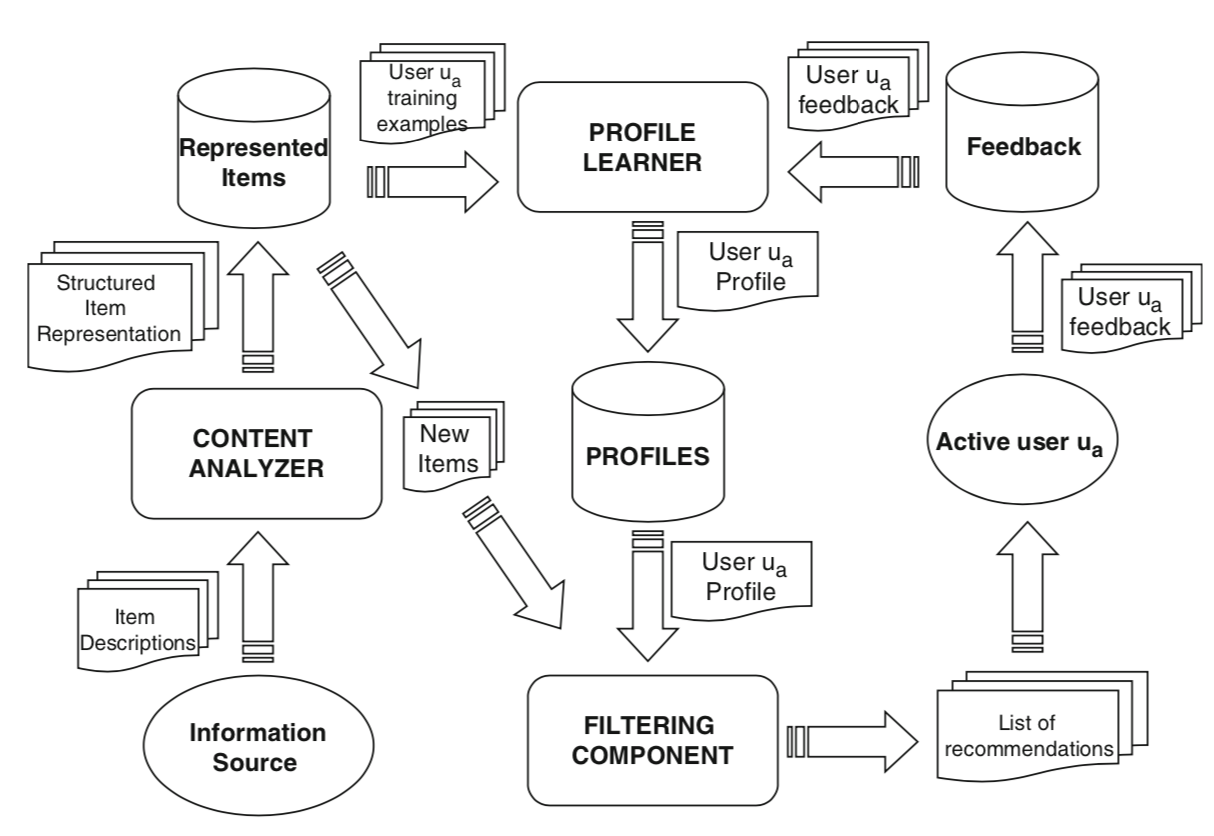
\includegraphics[width=\textwidth]{figures/HighLevelContentBased.png}
	\caption{High level architecture of a content based recommender  ~\parencite{de2015semantics}.}
	\label{fig:high-level-content-based}
\end{figure}



\begin{itemize}
\item CONTENT ANALYZER—The first part in the architecture is responsible for scraping or getting the data from  a source and saving them in a structured representation as items. If the data is a view data on a website, a scraper is needed to download and save them. However, if the desired input is metadata, then more advanced methods are needed to conduct an analysis. The output of this step is the input for the \textit{profile learner}.
\item PROFILE LEARNER—The profile learner module gets the learning data and trains the model or creates the user profiles, which generalizes from the learning data. Using the generalization strategy, the profile learner creates a profile that improves on user's positive and negative interactions with the items. For the case of this thesis, we both create profiles for users and items(talents). The profile learner also takes the advantage on enhancing the models with the human feedback after running on production mode.
\item FILTERING COMPONENT—The last part of the architecture is the filtering component. It takes the user and item profiles, runs an operation, which generates a relevancy score for each user-item pair. Lastly, the component returns a recommendation list. Generating the relevancy score is a different process for different kind of models.
\end{itemize}

All of these components are crucial to make a functioning content-based recommender system. As the system constantly waits for new items, the feedback process is critical and the retraining should happen regularly.


\subsubsection{Advantages and Drawbacks of Content-Based Filtering}

The advantages of content-based filtering against collaborative filtering are listed below \cite{de2015semantics}:

\begin{itemize}
	\item USER INDEPENDENCE—Content-based recommenders only need user profile for the relevant user. However, collaborative filtering recommenders require user profiles of all the other users so that it can suggest items based on nearest neighbors principle.
	\item TRANSPARENCY—Explanations on how the recommender system works can be provided by explicitly listing content features or descriptions that caused an item to occur in the list of recommendations. Those features are indicators to consult in order to decide whether to trust a recommendation. Conversely, collaborative systems are black boxes since the only explanation for an item recommendation is that unknown users with similar tastes liked that item;
	\item NEW ITEM—Content-based recommenders are capable of recommending items not yet rated by any user. As a consequence, they do not suffer from the first-rater problem, which affects collaborative recommenders which rely solely on users’ preferences to make recommendations. Therefore, until the new item is rated by a substantial number of users, the system would not be able to recommend it.
\end{itemize}

Nonetheless, content-based systems have several shortcomings:

\begin{itemize}
	\item LIMITED CONTENT ANALYSIS—Content-based techniques have a natural limit in the number and type of features that are associated, whether automatically or manually, with the objects they recommend. Domain knowledge is often needed, e.g., for movie recommendations the system needs to know the actors and directors, and sometimes, domain ontologies are also needed. No content- based recommendation system can provide suitable suggestions if the analyzed content does not contain enough information to discriminate items the user likes from items the user does not like. Some representations capture only certain aspects of the content, but there are many others that would influence a user’s experience. For instance, often there is not enough information in the word frequency to model the user interests in jokes or poems, while techniques for affective computing would be most appropriate. Again, for Web pages, feature extraction techniques from text completely ignore aesthetic qualities and additional multimedia information. Furthermore, CBRSs based on a string matching approach suffer from problems of:
	\begin{itemize}
		\item POLYSEMY, the presence of multiple meanings for one word;
		\item SYNONYMY, multiple words with the same meaning;
		\item MULTI-WORD EXPRESSIONS, the difficulty to assign the correct properties to
		a sequence of two or more words whose properties are not predictable from
		the properties of the individual words;
		\item ENTITY IDENTIFICATION or NAMED ENTITY RECOGNITION, the difficulty
		to locate and classify elements in text into pre-defined categories such as the names of persons, organizations, locations, expressions of times, quantities, monetary values, etc.
		\item ENTITY LINKING or NAMED ENTITY DISAMBIGUATION, the difficulty of determining the identity (often called the reference) of entities mentioned in text.
	\end{itemize}
	\item OVER-SPECIALIZATION — Content-based recommenders have no inherent method for finding something unexpected. The system suggests items whose scores are high when matched against the user profile, hence the user is going to be recommended items similar to those already rated. This drawback is also called lack of serendipity problem to highlight the tendency of the content-based systems to produce recommendations with a limited degree of novelty. To give an example, when a user has only rated movies directed by Stanley Kubrick, she will be recommended just that kind of movies. A “perfect” content-based technique would rarely find anything novel, limiting the range of applications for which it would be useful.
	\item NEW USER—Enough ratings have to be collected before a content-based rec- ommender system can really understand user preferences and provide accurate recommendations. Therefore, when few ratings are available, as for a new user, the system will not be able to provide reliable recommendations.
\end{itemize}

[4.3 Eger textten anlam cikarma falan yaparsan eklersin]
[4.4 Eger textten anlam cikarma falan yaparsan eklersin, bir oncekinin daha basiti ama iste insan olmadan halletme gibi]
[4.5 ayni sekilde]

\subsection{Conclusion}
[Biraz 4.6 dan alabilirsin ama hepsi alakali degil]



